%%%%%%%%%%%%%%%%%%%%%%%%%%%%%%%%%%%%%%%%%%%%%%%%%%%%%%%%%%%%%%%%%%%%%%%%
\chapter{Historical French Corpora}\label{chap:historical}
%%%%%%%%%%%%%%%%%%%%%%%%%%%%%%%%%%%%%%%%%%%%%%%%%%%%%%%%%%%%%%%%%%%%%%%%

\begin{center}
    \begin{minipage}{0.66\textwidth}
        \begin{small}
            In which we present a part of the work of \citet{grobol-etal-2022-bertrade} who put together a raw corpus for Medieval French intended to pre-train language models. We also present part of the work of \citet{gabay-etal-2022-from} who construct a \freemmax,a corpus for Early Modern French for the pre-training of language models, as well as \freemner an evaluation corpus annotated in named entity recognition. We also briefly present \freemlpm an evaluation corpus annotated in part-of-speech tagging.\footnotemark
        \end{small}
    \end{minipage}
    \vspace{0.5cm}
\end{center}

\footnotetext{Contributions: For the part of \citep{grobol-etal-2022-bertrade} presented in this chapter, I just helped with the statistics presented in table \ref{tab:texts_train} and figure \ref{fig:metadata}. For the part \citep{gabay-etal-2022-from} presented here, I helped in the crawling of some of the Wikisource transcriptions and some transcriptions found online. For the subsection \ref{freem_ner} I coded a script that allows to parse the corpus into a machine-readable format, find some common mistakes in annotations and generate the final split; I also made some manual corrections to the training corpus itself.}

Having extensively worked in Contemporary French corpora, we wanted to refocus and develop some historical French resources. As mentioned in the introduction of this thesis, this Ph.D. project was conceived and financed by ANR BASNUM (ANR-18-CE38-0003) project, whose main objective was to digitize and enrich Antoine Furetière's \emph{Dictionnaire Universel} (DU), in its 1701 version reviewed and corrected by Basnage de Beauval \citep{furetiere-1701-dictionnaire}, a text written in its entirety in Early Modern French. In Section \ref{data-freem} we develop resources for Early Modern French intended for both the pre-training and the evaluation of neural language models. This will allow us to develop, in the next Part, state-of-the-art models capable of conducting the dictionary enriching task originally planned by the BASNUM project.

Having said this, we also decided to participate in the curation of a small Medieval French corpus for the pre-training of a language model. Participating in this endeavor means that at the end of this chapter we will have developed resources for French covering a period going from the 9\textsuperscript{th} century to the present day, that is, we will have developed and curated textual resources for effectively all language states of French.

\section{Medieval French Corpus}
\label{sec-data}

This section describes the raw corpus of Medieval French we gathered in order to train unsupervised language models for Old French. To our knowledge, it is one of the largest such dataset gathered for Medieval French, although it remains quite small (\SI{55}{\mebi\byte} in total) relatively to the corpora usually used for pre-training contextual embeddings models.

We chose to include a few texts from the early Middle French period (14\textsuperscript{th} -15\textsuperscript{th}  c.) in this raw corpus, which brings a valuable complement of the prose documents that are lacking for Old French, while staying close enough to late Old French, the boundary between the two epochs being somewhat fuzzy. These texts precede the adoption of norms established by editors after the invention of Gutenberg's printing press. Middle French is more regular than Old French in some respects such as word order \citep{marchello-Nizia-etal-2020-grande} and less in others such as NP structure and pronouns system \citep{marchello-nizia-etal-1979-histoire}, but they share most of their lexicon and for these relatively early texts, the syntax is not too different from that of late Old French texts.

%Corpora
\begin{table}[thb]
    \centering
    \tablefontsize
    \begin{tabular}{l S[table-format=2.1]}
        \toprule
        {\textbf{Corpus}}                              & {\textbf{Size / \si{\mebi\byte}}} \\ %& {\textbf{\# texts}}
        \midrule
        BFM \citep{guillot-etal-2018-base}             & 20.7                              \\ %139
        AND \citep{rothwell-etal-2005-anglo}           & 17.2                              \\ %73
        NCA \citep{kunstmann-stein-2007-le}            & 9.7                               \\ %271
        Chartes Douai \citep{glessen-2003-elaboration} & 3.1                               \\ %1
        OpenMedFr \citep{wrisley-2018-the}             & 1.7                               \\ %19
        Geste \citep{camps-etal-2019-geste}            & 1.5                               \\ %32
        MCVF \citep{martineau-2008-un}                 & 1.4                               \\ %17
        Chartes Aube \citep{reenen-etal-2007-chartes}  & 0.2                               \\ %75
        \midrule
        Total                                          & 55.3                              \\ %627
        \bottomrule
    \end{tabular}
    \caption{Data collection}
    \label{tab:texts_train}
\end{table}

\begin{figure}[thb]
    \centering
    \begin{tikzpicture}
        \begin{axis}[
                xbar,
                colormap name=viridis,
                cycle list={
                        {color of colormap=200, draw=., preaction={fill=.}, pattern=grid},
                        {color of colormap=800, draw=., preaction={fill=.}, pattern=dots},
                    },
                font=\footnotesize,
                width=0.5\linewidth,
                yticklabel style={
                        xshift=0.5cm,
                        align=right,
                    },
                y axis line style = { opacity = 0 },
                xlabel = Datasize (\unit{\mebi\byte}),
                %axis x line       = none,
                tickwidth         = 0pt,
                ytick             = data,
                % enlarge y limits  = 0.15,
                % enlarge x limits  = 0.2,
                symbolic y coords = {Legal, Historical, Didactic, Religious, Literature},
                nodes near coords,
                nodes near coords style={black},
                legend style={at={(0.95,0.6)}},
                reverse legend,
            ]
            \addplot
            coordinates {(13.3321,Literature) (4.35204,Religious)
                    (4.35204,Didactic) (0.687576,Historical) (0,Legal)};
            \addlegendentry{Verse}
            \addplot
            coordinates {(2.352817,Literature) (4.433186,Religious)
                    (3.041925,Didactic) (8.362256,Historical) (15.705591,Legal)};
            \addlegendentry{Prose}
            % 			\legend{Verse,Prose}
        \end{axis}
    \end{tikzpicture}
    \caption{Distribution of form and domain, gathered from documents metadata and manual annotation.}
    \label{fig:metadata}
\end{figure}

Medieval French has many factors of variation: language evolution, dialects, domains, forms of text (verse or prose) and lack of standard. Our dataset gives us a representation of Medieval French that is as accurate and diversified as possible, given the limited amount of material that survived to these days.
The detailed instructions to replicate this dataset are described in the Appendix \ref{subsec:collectdata}. No particular processing is done on the original documents.

In order to get a sound evaluation of the contextual embeddings trained with this dataset, we filter out the documents that are also present in the SRCMF treebank used for evaluation purposes in section \ref{sec-experiments}.\footnote{As noted by \citet{gururangan-etal-2020-dont}, pre-training on task specific data provides an additional boost, this would muddle our results, since our objective here is not so much task optimization as embeddings benchmarking.} The resulting corpus is quite heterogeneous: legal texts and verse literature are in the majority, whereas other domains, such as historical and didactic texts, are under-represented, as can be seen in \cref{fig:metadata}.


\section{Early Modern French Corpora}\label{data-freem}

For the past few years, we have been involved in the development of linguistic resources for Early Modern French. The initiative, called \textsc{FreEM} (which stands for \emph{FREnch Early Modern}), aims to collect the corpora required for various NLP tasks such as lemmatization, POS tagging, linguistic normalization and named entity recognition. Two of these corpora are introduced here: \freemmax (see Section~\ref{freem_max}) and \freemlpm (see Section~\ref{freem_lpm}).

\subsection{\texorpdfstring{\freemmax}{FREEM max}}\label{freem_max}

Usable historical documents are difficult to find because, as previously mentioned, they are more rare than contemporary ones; editors tend to normalize the language (\emph{i.e.}~use the spelling conventions of contemporary French, see~\citep{gabay-2014-pourquoi}), transcriptions are not (always) distributed in a digital format. \freemmax \citep{gabay-etal-2022-FreEM} is an attempt to solve this problem, and the aim of this dataset is to group together the largest number of texts possible written in Early Modern French.

The texts we have curated have a variety of sources, which can be grouped into three main types:
\begin{itemize}
    \item Two institutional datasets have been used and are non open-sourced:
          \begin{itemize}
              \item \textsc{Frantext} \emph{intégral} \citep{atilf-1998-frantext}, the biggest database of French texts (only the texts between 1500 and 1800), a very small portion of which is open access: \textsc{Frantext} \emph{Démonstration} \citep{atilf-1998-frantext-d};
              \item \emph{Electronic Enlightenment} \citep{bodleian-2008-electronic}, an online collection of edited correspondences of the Early Modern period;
          \end{itemize}
    \item Several come from research projects distributing transcriptions online:
          \begin{itemize}
              \item The \emph{Antonomaz project},  French \emph{mazarinades} (\url{https://cahier.hypotheses.org/antonomaz});
              \item The II.B section (in French) of the \emph{Actis Pacis Westphalicae}, diplomatic letters for the Peace of Westphalia (\url{http://kaskade.dwds.de/dstar/apwcf/});
              \item The Bibliothèques virtuelles humanistes, 16\textsuperscript{th}\,c.~French literature (\url{http://www.bvh.univ-tours.fr});
              \item The \emph{Corpus électronique de la première modernité}, 17\textsuperscript{th}\,c.~French literature (\url{http://www.cepm.paris-sorbonne.fr})
              \item The \emph{Condé} project, \emph{coutumiers normands} (\url{https://conde.hypotheses.org})
              \item The Corpus Descartes, works of René Descartes (\url{https://www.unicaen.fr/puc/sources/prodescartes/});
              \item The \emph{Bibliothèque dramatique} of the CELLF, 17\textsuperscript{th}\,c.~French plays (\url{http://bibdramatique.huma-num.fr});
              \item The \emph{Fabula numerica} project, French fables (\url{https://obvil.sorbonne-universite.fr/projets/fabula-numerica});
              \item The \emph{ Fonds Boissy}, plays of Louis de Boissy (\url{https://www.licorn-research.fr/Boissy.html});
              \item The \emph{Mercure Galant} project, the famous French \emph{gazette} and literary magazine between 1672 and 1710 (\url{https://obvil.sorbonne-universite.fr/corpus/mercure-galant});
              \item The \emph{Rousseau online} project, works of Jean-Jacques Rousseau (\url{https://www.rousseauonline.ch});
              \item The \emph{Sermo} project, sermons of the 16\textsuperscript{th} and 17\textsuperscript{th}\,c. (\url{http://sermo.unine.ch});
              \item The \emph{Théâtre classique} project, 17\textsuperscript{th} and 18\textsuperscript{th}\,c.~French plays (\url{http://www.theatre-classique.fr});
          \end{itemize}
    \item Additional sources come from researchers who kindly accepted to offer their personal transcriptions or data scrapped by our team:
          \begin{itemize}
              \item Transcriptions by Anne-Élisabeth Spica (17\textsuperscript{th}\,c. French novels);
              \item Transcriptions found on \emph{Wikisource} (\url{https://fr.wikisource.org});
              \item Transcriptions (ePub files) found on \emph{Gallica} (\url{https://gallica.bnf.fr});
              \item Transcriptions found on various websites online.
          \end{itemize}
\end{itemize}

\begin{table}[ht]
    \centering\small
    \resizebox{\linewidth}{!}{
        \begin{tabular}{lrrlr}
            \toprule
            Origin                      & \#Tokens  &  & Origin                                               & \#Tokens    \\
            \midrule
            Spica corpus                & 691,467   &  & \textsc{Frantext} \emph{intégral} ($>$1500, $<$1800) & 60,018,390  \\
            Antonomaz project           & 119,194   &  & \textsc{Frantext} \emph{intégral} ($>$1800)          & 71,504,440  \\
            Acta Pacis Westphlicae II B & 2,463,047 &  & \textsc{Frantext} \emph{Démonstration}               & 1,255,454   \\
            Bibliothèque Bleue          & 776,838   &  & Gallica                                              & 5,212,333   \\
            BVH                         & 2,434,657 &  & Boissy project                                       & 438,215     \\
            CEPM                        & 2,707,432 &  & Mercure galant                                       & 5,427,469   \\
            Condé project               & 3,173,845 &  & Rousseau Online project                              & 2,428,587   \\
            Descartes                   & 1,025,337 &  & Scrapping                                            & 1,936,835   \\
            CELLF                       & 1,873,772 &  & Sermo project                                        & 529,647     \\
            Electronic enlightenment    & 6,568,047 &  & Théâtre classique project                            & 13,916,169  \\
            Fabula project              & 145,978   &  & Wikisource                                           & 996,329     \\
            \midrule
            \textbf{TOTAL}              &           &  &                                                      & 185,643,482 \\
            \bottomrule
        \end{tabular}
    }
    \caption{Breakdown of the \freemmax corpus by text origin.}
    \label{tab:my_label}
\end{table}

\begin{figure}[ht]
    \centering
    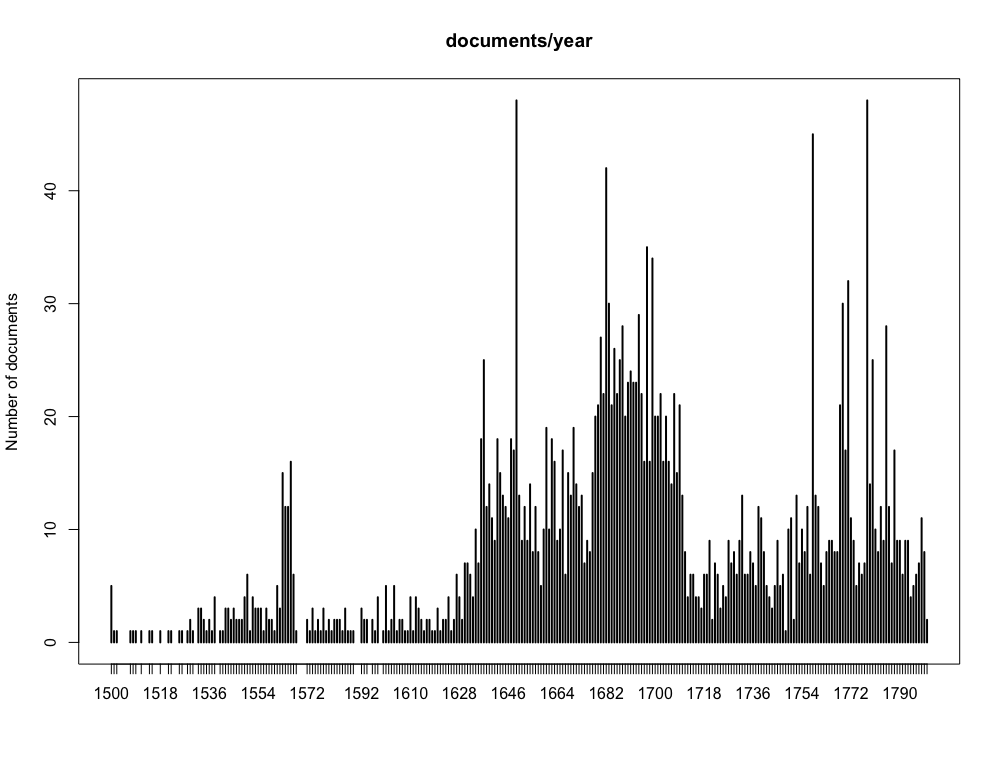
\includegraphics[width=0.75\linewidth]{static/media/mod_eval/dalembert/desc_DalemBERT.png}
    \caption{Distribution of the documents in the \freemmax corpus per year}
    \label{fig:FreEMmax_desc}
\end{figure}

Additional data for later states of the language, up to the 1920's (mainly from FRANTEXT \emph{intégral}), are also provided for two main reasons: on the one hand, it is common to normalize Early Modern French into Contemporary French \citep{gabay-2014-pourquoi} because of the linguistic proximity between these the two states of the language, and on the other hand, it helps to collect (precious) additional data to avoid ending up with too small of a corpus for our needs.

The final result is far from being balanced or representative (see Figure~\ref{fig:FreEMmax_desc}). 16\textsuperscript{th}\,c. French documents are under-represented, as well as 18\textsuperscript{th}\,c.~literature. The 17\textsuperscript{th}\,c. is clearly over-represented, especially its second half---probably one of the most important of French literature, which could explain this situation (on top of our personal interest for this specific period).

As some texts are still (partially) protected by restrictive licenses, the \freemmax corpus exists in both open and non-open versions, only the open one being distributed.\footnote{\url{https://freem-corpora.github.io/corpora/max/}} In order to limit the impact of licenses forbidding the modification of files, we have designed a pipeline to distribute the data as it was found and recreate it (see Figure~\ref{fig:pipeline}).

Metadata is prepared manually in order to have the same categories for each document, whatever its origin. As well as the author, the title and the date (where relevant), we also provide the genre (``theater''), sometimes a subgenre (``tragedy''), the linguistic status (normalized or not) and the license attached to the transcription.

\begin{figure}[ht]
    \centering
    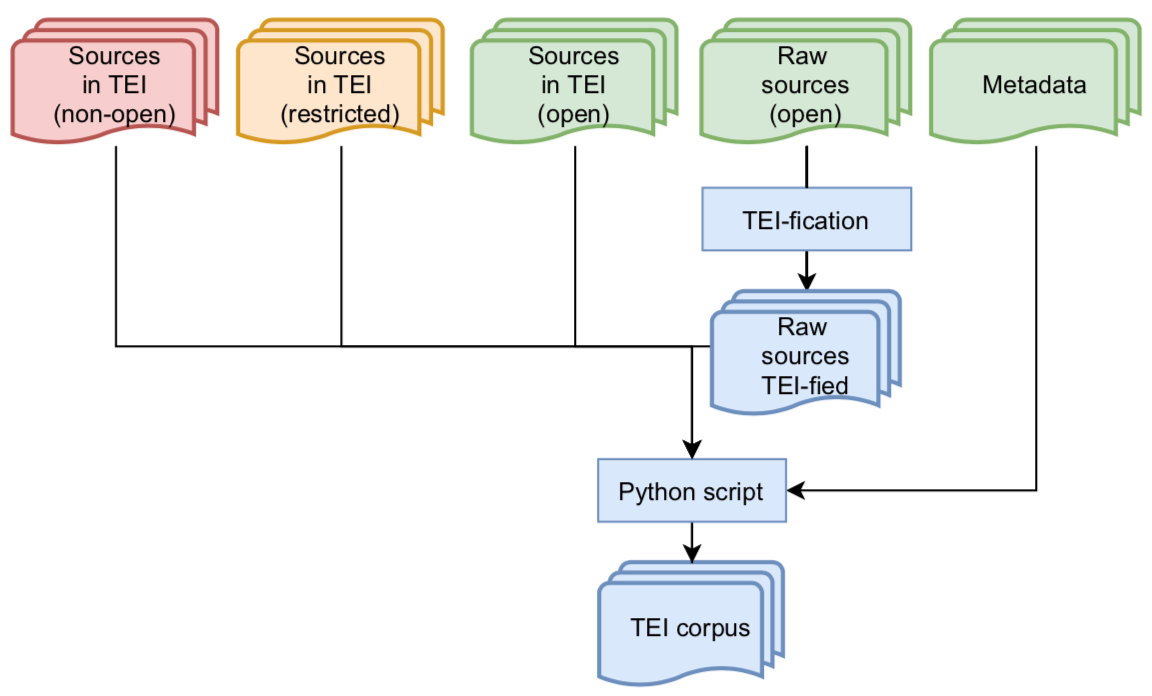
\includegraphics[width=0.75\linewidth]{static/media/mod_eval/dalembert/corpus_trans.png}
    \caption{\freemmax compilation pipeline. All files are kept in their original format. Metadata is manually prepared in separate files in order to automatically transform and clean (in blue) all the available documents into XML TEI files following the same encoding. It allows us to distribute open data (in green) but also data distributed with restrictions regarding the modification of the original format (in orange). Non-open texts (in red) are not distributed.}
    \label{fig:pipeline}
\end{figure}

\subsection{\texorpdfstring{\freemlpm}{FREEM LPM}}\label{freem_lpm}

The \freemlpm \citep{gabay-etal-2020-standardizing} stands for \emph{Lemma, POS tags, Morphology}. The POS-annotated data, is a mixture of two different sources. On the one hand, there is the \emph{CornMol} corpus \citep{camps-etal-2021-corpus}, made up of normalized 17\textsuperscript{th}\,c.~French comedies. On the other hand, there is a gold subset of the \emph{Presto} corpus \citep{blumenthal-etal-2017-presto}, made up of texts of different genres written during the 16\textsuperscript{th}, 17\textsuperscript{th} and 18\textsuperscript{th}\,c., which have previously used to train annotation tools \citep{diwersy-etal-2017-ressources}, and was heavily corrected by us to match our annotation principles \citep{gabay-etal-2020-manuel}.

On top of traditional in-domain tests, an out-of-domain testing dataset was prepared to control the capacity of the model to generalize to other genres and periods. Centuries covered are the 16\textsuperscript{th}, 17\textsuperscript{th}, 18\textsuperscript{th}, 19\textsuperscript{th} and 20\textsuperscript{th}. There are two test sets for each century: one made up only of theater, the other of everything but theater. Each test set comprises 10 short samples (c.\,100 tokens), as representative as possible of the linguistic production of the century (female and male authors, decade of publication, genre, etc.).

All the data from \freemlpm (but almost none of the out-of-domain) can be found in \freemmax.

\subsection{\texorpdfstring{\freemner}{FREEM NER}}\label{freem_ner}

\begin{figure}[!ht]
    \centering
    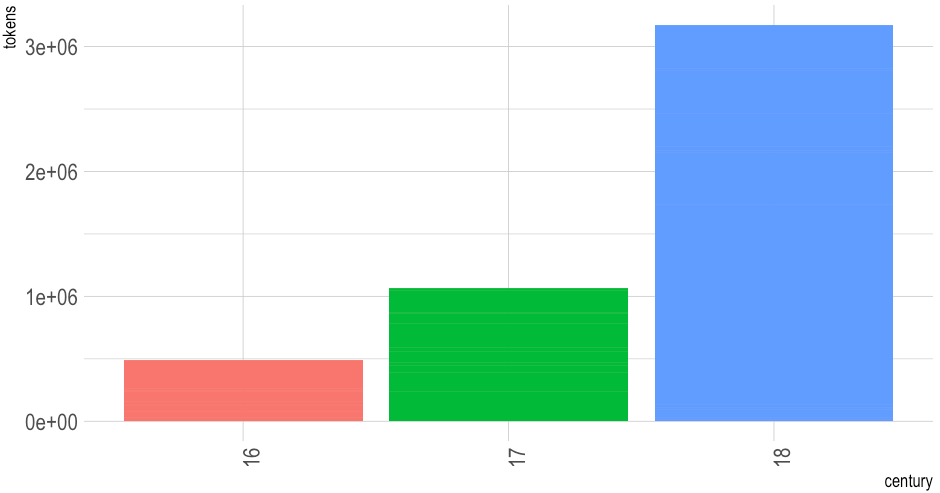
\includegraphics[width=0.6\linewidth]{static/media/mod_eval/dalembert/distribution_tokens_corpus.png}
    \caption{Number of tokens per century.}
    \label{fig:description}
\end{figure}

Rather than designing a new corpus, we have decided to use a subpart of the ``core corpus'' of the \textit{Presto} project~\citep{blumenthal-etal-2017-presto}, namely the text written during the French \textit{Ancien Régime} (c.15\textsuperscript{th}-18\textsuperscript{th}\,c., i.e. 34 texts).\footnote{A text has been withdrawn: the \textit{Histoire d'un voyage faict en la terre du Brésil} by Jean de Léry, the transcription being too faulty to be able to correctly annotate the document.} This choice is driven by our will to limit the number of annotated corpora for historical French, the same set of documents having already been abundantly corrected to train a lemmatizer~\citep{gabay-etal-2020-standardizing}, but also to avoid a complex selection of works supposed to ensure a relative representativeness of literary documents from the \textit{Ancien Régime}, already perfectly done by our colleagues.

The number of genres covered is very large: poetry, drama, novel, correspondence, grammar, philosophy, short stories, encyclopedic literature, etc. and guarantees, here again, a reasonable representativeness of the range of possibilities of \textit{Belles-Lettres}.\footnote{We do not offer a detailed description of the genres covered, these overlapping easily: poetry can be theological, political correspondence, etc.} The corpus is balanced regarding the distribution per century (approx\,10/century) but not regarding the length of the texts, which increases over time (cf.\,fig.~\ref{fig:description}), following a possible trend in literature.

\subsubsection{Annotation}

\begin{table}[!htp]
    \centering\small
    \begin{tabular}{llllll}
        %{@{}p{0.15\linewidth}p{0.15\linewidth}p{0.15\linewidth}p{0.15\linewidth}p{0.15\linewidth}p{0.15\linewidth}@{}}
        \rowcolor{lightgray}
        \multicolumn{3}{c}{Person}                                                                   & \multicolumn{3}{c}{Function}                                                              \\
        \multicolumn{3}{c}{\begin{tabular}{cc} \texttt{pers.ind} & \texttt{pers.coll} \end{tabular}} &
        \multicolumn{3}{c}{\begin{tabular}{cc} \texttt{func.ind} & \texttt{func.coll} \end{tabular}}                                                                                             \\
        \rowcolor{lightgray}
        \multicolumn{3}{c}{Location}                                                                 & \multicolumn{3}{c}{Production}                                                            \\
        \texttt{loc.adm.town}                                                                        & \texttt{loc.phys.geo}                      & \texttt{loc.fac}                           &
        \texttt{prod.art}                                                                            & \texttt{prod.rule}                         & \texttt{prod.object}                         \\
        \texttt{loc.adm.reg}                                                                         & \texttt{loc.phys.hydro}                    & \texttt{loc.oro}                           &
        \multicolumn{3}{c}{\begin{tabular}{cc}  &  \end{tabular}}                                                                                                                                \\
        \texttt{loc.adm.nat}                                                                         &                                            &                                            &
        \multicolumn{3}{c}{\begin{tabular}{cc}  &  \end{tabular}}                                                                                                                                \\
        \texttt{loc.adm.sup}                                                                         &                                            &                                            &
        \multicolumn{3}{c}{\begin{tabular}{cc}  &  \end{tabular}}                                                                                                                                \\
        \rowcolor{lightgray}
        \multicolumn{2}{c}{Organization}                                                             & \multicolumn{2}{c}{Time}                   &
        \multicolumn{1}{c}{Event}                                                                    &
        \multicolumn{1}{c}{Quantity}                                                                                                                                                             \\
        \texttt{org.adm}                                                                             & \texttt{org.ent}                           & \multicolumn{2}{c}{\texttt{time.date.abs}} &
        \multicolumn{1}{c}{\texttt{event}}                                                           &
        \multicolumn{1}{c}{\texttt{amount}}                                                                                                                                                      \\
        \multicolumn{2}{c}{}                                                                         & \multicolumn{2}{c}{\texttt{time.date.rel}} &
        \multicolumn{2}{c}{}                                                                                                                                                                     \\
    \end{tabular}
    \caption{Types (in gray) and subtypes taken from the \emph{Quaero} typology.}
    \label{tab:types}
\end{table}

Because two important historical corpora presented \textit{supra} (\textit{Quaero} and \textit{Impresso}) have chosen to follow the \textit{Quaero} annotation guide~\citep{rosset-etal-2011-entites}, it seemed logical to use this same typology. Because our texts and interests diverge from those of the aforementioned corpora, only some types and subtypes have been kept (cf.\,tab.~\ref{tab:types}) from the \textit{Quaero} annotation scheme. The details of our annotation choices can be found in a dedicated annotation manual~\citep{gabay-etal-2020-manuel}.

\begin{table}[!htp]
    \centering\scriptsize
    \begin{tabular}{llrrrrrr}
        \toprule
        Token     & Lemma    & POS & COARSE & FINE       & FINE-COMP    & NESTED        & Wikidata ID \\
        \midrule
        Les       & le       & Da  & O      & O          & O            & O             & \_          \\
        allemands & allemand & Nc  & O      & O          & O            & O             & \_          \\
        élurent   & élire    & Vvc & O      & O          & O            & O             & \_          \\
        pour      & pour     & S   & O      & O          & O            & O             & \_          \\
        empereur  & empereur & Nc  & B-pers & B-pers.ind & B-comp.title & O             & Q438435     \\
        Rodolphe  & Rodolphe & Np  & I-pers & I-pers.ind & B-comp.name  & O             & Q438435     \\
        duc       & duc      & Nc  & I-pers & I-pers.ind & B-comp.title & O             & Q438435     \\
        de        & de       & S   & I-pers & I-pers.ind & I-comp.title & O             & Q438435     \\
        Suabe     & Souabe   & Np  & I-pers & I-pers.ind & I-comp.title & B-loc.adm.reg & Q438435     \\
        \bottomrule
    \end{tabular}
    \caption{NERC Fine-Grained annotation avec EL}
    \label{tab:data}
\end{table}

The annotated texts are available in multi-columns \texttt{tsv} files (cf.\,tab.~\ref{tab:data}). Each token has a lemma (manually corrected) and a POS (produced by the \textit{Presto} project, non-systematically corrected but fairly reliable) using the MULTEXT tag set. We propose a coarse-grained annotation for high-level entity types and fine-grained annotation using subtypes using the following syntax:
\begin{quote}
    \texttt{\ora{BIO}}-\texttt{\purp{TYPE}}.\texttt{\teal{SUBTYPE}} \\
    \textit{For instance: } \texttt{\ora{B}}-\texttt{\purp{loc}}.\texttt{\teal{adm.town}}
\end{quote}

\noindent Subtypes are sometimes simple (\texttt{B-org.\teal{town}}) sometimes double (\texttt{B-loc.\teal{phys.geo}}), depending of the complexity of the entity to annotate. Nested entities (\textit{i.e.} an entity in an entity, such as a place name in a person name in \textit{Henri d'\textbf{Angleterre}}, ``Henry of England``) follow exactly the same syntax, and components a similar one, using six transverse elements:

\begin{itemize}
    \item \texttt{name} to annotate tokens that are names (\textit{Louis}, \textit{Philippe}\dots)
    \item \texttt{title}  to annotate tokens that are titles (\textit{sieur}, \textit{duc}, \textit{abbé}\dots)
    \item \texttt{qualifier} to annotate tokens that are adjectives (\textit{l'Inde \textbf{orientale}}, \textit{l'Arabie \textbf{heureuse}}, \textit{la mer \textbf{athlantique}}, \textit{l'\textbf{ancienne} Colchide})… but also the generation (\textit{Henri \textbf{IV}}) or a cardinal position
    \item \texttt{kind} to annotate tokens that are hyperonyms (\textit{l'\textbf{Empire} de Constantinople}, \textit{la \textbf{mer} du Japon}
    \item \texttt{unit} to annotate tokens that are units (meters, league, inches, pounds…)
    \item \texttt{val} to annotate tokens that are values (a number) that is linked to a unit to annotate an \texttt{amount}.
\end{itemize}

\begin{figure}[!htp]
    \centering
    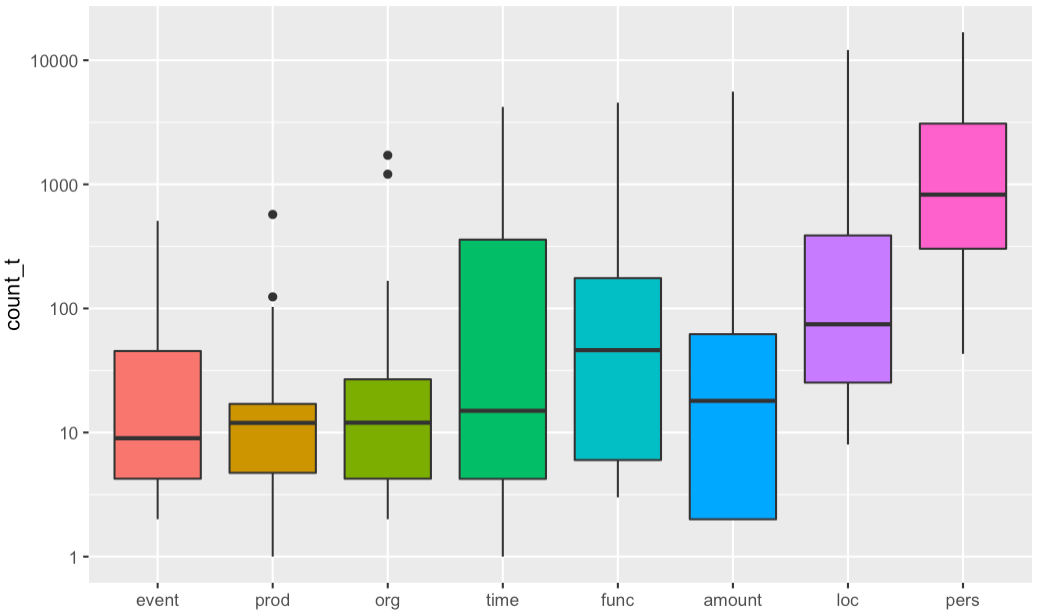
\includegraphics[width=0.75\linewidth]{static/media/mod_eval/dalembert/corpus_desc_1.png}
    \caption{Number of entities (\textit{$\log_{10}$} scale) per category.}
    \label{fig:repartition}
\end{figure}

We have decided not to annotate metaphorical uses differently or in a separate column: everything is annotated in a literal sense. Thus, in \textit{\textbf{France} goes to war}, \textit{France} is labelled \texttt{loc.adm.nat} (\textit{i.e.} the country) and not \texttt{org.adm} (\textit{i.e.} the French government).

We have also started a first phase of semantic annotation, using Wikidata~\citep{vrandecic-krotzsch-2014-wikidata} identifiers, which remains imperfect. Due to the complexity of analyzing certain entities, in particular personal names (e.g. \textit{Pope John}), it was decided to annotate them only very marginally, only in the event of the absence of ambiguity (e.g. \textit{Pope John V}). The annotation of place names, on the other hand, is more advanced and almost exhaustive.

A first layer of annotation was made using regular expressions, before moving on to a manual correction phase. Given the size of the corpus, it is obvious that each token has not been checked, and that the final result does not claim to be perfect. Occasional checks, however, concluded that the annotation was of high enough quality to move on to the training phase. All the annotation work was carried out by a single person, in order to ensure the consistency of the data. The structure of the file and the form of the tags was controlled by a specific parser, designed specifically for this corpus. Figure \ref{fig:repartition} shows the distribution of the coarse entity categories throughout \freemner on a logarithmic scale. For more detail please refer to figures \ref{fig:entities-by-text} and \ref{fig:entity-type-per-text} in the appendix.

\section{Conclusion}

In this chapter we have presented two raw textual corpora for historical French intended to be used in the pre-training of state-of-the-art language models, one for Medieval French and another one for Early Modern French. These corpora will be used in the next par of this thesis to produce two language models in order to tackle the textual enriching task proposed by the BASNUM project. As these two corpora are in fact quite general and diverse, we believe that the models they will produce will allow researcher in Digital Humanities to enrich and better study not only for the \emph{Dictionnaire Universel}, but also any other text in Early Modern or Medieval French.

We have also presented a NER annotated corpus in Early Modern French, that will allow not only to evaluate our language models for Early Modern French in the upcoming part of the thesis, but also to produce a general ready-to-use state-of-the-art model for NER in Early Modern French.
